% -*- root: ../main.tex -*-
\chapter{Design\label{chap:design}}

\paragraph{Abstract} In this chapter we cover the description of the theory used. As we mentioned before is the linked list theory, but one may implement this theory in many different ways. 

Once the theory we are working with is defined, we will expose the goals we intend to prove and which are the intermediate steps to prove the safety of this theory.


\section{Program correctness}


We are finally ready to apply this concepts to a real word problem. In this \thisworkm we apply those concepts to prove some properties of programs.
%
The remaining task is to define the framework and the conventions we use to prove formally properties of programs.

The way of proving correctness is by proving properties. 
%
There are \concept{liveness}, \concept{safety} and \concept{functional} properties. 
%
Safety properties refer, informally, to "bad things never happens". Proving \textit{ variable x is never 0 } is a safety property. 
%
Proving its validity can assure that a division by zero error does never occur. 
%
Whether a program finishes or not is a liveness property and receiving an output for a concrete input is a functional property. 

This properties are written in some logic. Liveness properties need \gls{LTL} but \gls{FOL} is enough to prove safety properties. 
%
As the properties are expressed formally in logic, it is necessary to define a formal representation of a program.


\label{def:SPL}
% -*- root: ../main.tex -*-
\subsection{Formal representation of a program}

This \gls{SPL} and its formal representation is the language chosen to write the programs to be formally verified.
%
It has been chosen by \citep{thesisAle} because its simplicity and \doubt{expressiveness} in order to write concurrent programs. 
%
Because its simplicity it is a great option to do formal verification with it.


\subsubsection{Preliminaries (Notation, definition)}

One can consider a program as a series of state changes. There are some variables, we execute one line of the program and some of those variables changes and some others don't. Thus, we can consider any program as a graph of states with some ways. For example, lets take a very simple program:
%
\[
	\begin{array}{l@{\hspace{0.3em}}c@{\hspace{1em}}l}
	\hline
		l_1 & : & \mathtt{x := -2} \\
		l_2 & : & \mathtt{\textbf{if } (x<0)} \\
		l_3 & : & \mathtt{\;\;x = 2x} \\
		l_4 & : & \mathtt{\textbf{...}}\\
	\hline
	\end{array}
\]
\label{simple:example}

This simple program doesn't do anything interesting, but it is useful to illustrate.
%
In figure \ref{ex:simpleExample} the directed graph of states is shown.

\begin{figure}[hbtp]
\label{ex:simpleExample}
\centering
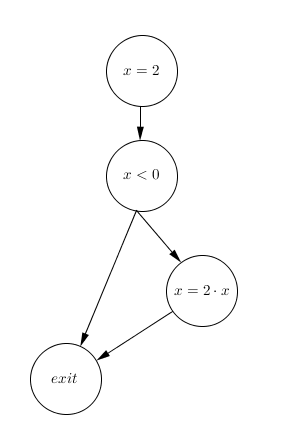
\includegraphics[scale=0.6]{graphics/simpleExample.png}
\caption{Directed graph of the program \ref{simple:example}}
\end{figure}


In the execution of this program, it is not possible to execute line 3 just after line 1 skipping line 2. We need to go line by line, respecting the execution flow. 
This is represented by the variable \pc (\concept{Program\IS counter}). This variable indicates the line to execute next.

So the state of the program at the beginning is 
%
\[ \pc = 1\]
%
This formula give all the information we have of the execution state. 
We know the \pc\; and the state and value of all variables (there are no more variables than \pc).

Now we need to define the step. 
%
How can we represent the execution of a line.
%
We need to use \concept{post-state} variables. 
%
We define the prime version of any variable to refer that same variable after the execution of the line (transition). 
%
Going back to the example, we have:
%
\[
\pc = 1 \andcond \pc'=2 \andcond x'=2 
\]

We have a post-state program counter ($\pc'=2$) and some post-state variables. 
%
As the execution of the assignment the variable $x$ takes a value (independently of the value in the pre-state), then $x'=2$ (regardless what value $x$ had). 

The next step could be
\[
\pc = 2 \andcond x'=x \andcond 	\pc'=?
\]

Where ? depends on the validity of the \textit{if} condition. 

This steps we have illustrated are called transition relations.

\begin{defn}[Transition relation]
A transition relation is the formula that define the step from one state of the program to another.  
\end{defn}

With this simple example, we have shown what a program counter and what a transition relation are. Now we can define the possible instructions a program may have.\footnote{We have just took the set of instructions the programs we are going to proof have.}

\subsubsection{Possible instructions}
As we are going to work with programs used by more than one thread, we need one program counter for each thread executing. 
%
We parametrize the program counter. 
%
This is, defining the \textbf{program counter} as a \textbf{function} that given a thread, returns its program counter. 
%
We could have define as one variable per thread, but it would be equivalent. 

For this definitions we use the letter $T$ to refer a particular thread.

\begin{description}
\item [Assignments:]
		The transition relation for a variable assignment consists of the 
		update of the program counter for the running thread and the 
		corresponding modification to the variable being assigned.
%
			\[
			\begin{array}[t]{p{8em}@{\hspace{6em}}p{\longtablesize}}
				\hline
				Statement & Transition relation \\ \hline\hline
				$\begin{array}[t]{l@{\hspace{0.3em}}c@{\hspace{1em}}l}
					l_1 & : & \mathtt{v := 2} \\
					l_2 & : & \mathtt{\cdots}
				\end{array}$
				&
				$\begin{array}[t]{ll}
					 \pc(T) = l_1 \andcond
					 \pc'(T) = l_2 \andcond
					 \mathtt{v}' = 2
				 \end{array}$ \\ 
				 \hline
			\end{array}
			\]
%
	\item [Pointer access:]
		Structure fields are accessible through the pointer operator \pointsto.
%
		There are two possible scenarios for the use of pointers, depending on 
		whether the statement accesses or modifies a structure field.
%
		We present now the semantics for both cases.
%
		The first case corresponds to the access of a structure field through an 
		address pointer.
%
\[
\begin{array}[t]{p{8em}@{\hspace{6em}}p{\longtablesize}}
	\hline
	Statement & Transition relation \\ \hline\hline
	$\begin{array}[t]{l@{\hspace{0.3em}}c@{\hspace{1em}}l}
		\ell_1 & : & \mathtt{v := a \pointsto field} \\ \\
		\ell_2 & : & \mathtt{\cdots}
	\end{array}$
	&
	$\begin{array}[t]{ll}
		 \pc(T) = \ell_1 \andcond
		 \pc'(T) = \ell_2 \andcond \\
		 \mathtt{v}' = \heap[\mathtt{a}].\mathtt{field}
	 \end{array}$ \\
	 \hline
\end{array}
\]
%
		The second case corresponds to the modification of a structure field using 
		an address pointer.
%
		Note how, in the second case, all structures (except the one pointed by 
		$\mathtt{b}$) remain unchanged.
%
		Also, all fields of the structure pointed by $\mathtt{b}$ remain unmodified 
		except for $\mathtt{field_n}$.
%
		\[
		\begin{array}[t]{p{8em}@{\hspace{6em}}p{\longtablesize}}
						\hline
						Statement & Transition relation \\ \hline\hline
						$\begin{array}[t]{l@{\hspace{0.3em}}c@{\hspace{1em}}l}
							\ell_1 & : & \mathtt{b \pointsto field_n := a} \\ \\ \\ \\
							\ell_2 & : & \mathtt{\cdots}
						\end{array}$
						&
						$\begin{array}[t]{ll}
							\pc(T) = \ell_1 \andcond \pc'(T) = \ell_2 & \andcond \\
							\heap' = \heap \{ \mathtt{b} \leftarrow c \} & \andcond \\
							c.\mathtt{field_n} = \mathtt{a} & \andcond \\
							\bigwedge\limits_{i \neq \mathtt{n}} c.\mathtt{field}_i = 
							\heap[\mathtt{b}].\mathtt{field}_i
						\end{array}$\\ \hline
			\end{array}
		\]

	\item [Conditionals:]
		We present now the two possible kinds of conditional statements in 
		SPL.
%
		In the first case, if condition $c$ does not hold, the execution 
		proceeds from the statement following the end of the conditional.
%
		\[
        \begin{array}[t]{p{8em}@{\hspace{6em}}p{\longtablesize}}
				\hline
				Statement & Transition relation \\ \hline\hline
				$\begin{array}[t]{l@{\hspace{0.3em}}c@{\hspace{1em}}l}
					\ell_1 & : & \mathtt{\textbf{if } c \textbf{ then }} \\ \\
					\ell_2 & : & \mathtt{\cdots} \\
						&& \mathtt{\vdots} \\
					\ell_n & : & \mathtt{\textbf{end if}} \\
					\ell_{n+1} & : & \mathtt{\cdots}
				\end{array}$
				&
				$\begin{array}[t]{ll}
					(\pc(T) = \ell_1 \andcond \;\;\mathtt{c} \andcond \pc'(T) = \ell_2) \; \Or \\
					(\pc(T) = \ell_1 \andcond \lnot \mathtt{c} \andcond \pc'(T) = \ell_{n+1})
				 \end{array}$ \\ \hline
			 \end{array}
		 \]
%
		In the second case, if condition $c$ does not hold, the execution 
		continues at the first statement in the \textbf{else} section of the 
		conditional statement.
%
		\[
				\begin{array}[t]{p{8em}@{\hspace{6em}}p{\longtablesize}}
				\hline
				Statement & Transition relation \\ \hline\hline
				$\begin{array}[t]{l@{\hspace{0.3em}}c@{\hspace{1em}}l}
					\ell_1 & : & \mathtt{\textbf{if } c \textbf{ then }} \\ \\
					\ell_2 & : & \mathtt{\cdots} \\
					\mathtt{\vdots} \\
					\ell_n & : & \mathtt{\textbf{else}} \\
					\ell_{n+1} & : & \mathtt{\cdots} \\
					\mathtt{\vdots} \\
					\ell_m & : & \mathtt{\textbf{end if}} \\
					\ell_{m+1} & : & \mathtt{\cdots}
				\end{array}$
				&
				$\begin{array}[t]{ll}
					(\pc(T) = \ell_1 \andcond \;\;\mathtt{c} \andcond \pc'(T) = \ell_2) \; \Or \\
					(\pc(T) = \ell_1 \andcond \lnot \mathtt{c} \andcond \pc'(T) = \ell_{n+1})
						& \text{for line } \ell_1 \\ \\ \phantom{\vdots} \\

						\pc(T) = \ell_n \andcond \pc'(T) = \ell_{m+1} & \text{for line } \ell_n
				 \end{array}$ \\ \hline
			\end{array}
		\]
%
	\item [Loops:]
		We consider the only loop statement available in SPL which executes 
	the statements in the body as long as the loop condition holds.
%
		\[
				\begin{array}[t]{p{8em}@{\hspace{6em}}p{\longtablesize}}
				\hline
				Statement & Transition relation \\ \hline\hline
				$\begin{array}[t]{l@{\hspace{0.3em}}c@{\hspace{1em}}l}
					\ell_1 & : & \mathtt{\textbf{while } c \textbf{ do }} \\
					\ell_2 & : & \mathtt{\cdots} \\
					\mathtt{\vdots} \\
					\ell_n & : & \mathtt{\textbf{end while}} \\
					\ell_{n+1} & : & \mathtt{\cdots}
				\end{array}$
				&
				$\begin{array}[t]{ll}
						(\pc(T) = \ell_1 \andcond \;\;\texttt{c} \andcond \pc'(T) = \ell_2) \; 
						\Or \\
						(\pc(T) = \ell_1 \andcond \lnot \texttt{c} \andcond \pc'(T) = 
					\ell_{n+1})
					& \text{for line $\ell_1$} \\ \\
					\pc(T) = \ell_n \andcond \pc'(T) = \ell_1 &
						\text{for line $\ell_n$}
				 \end{array}$ \\ \hline
			 \end{array}
		\]
%
			\item [Non deterministic choice:]
		The transition relation for the non-deterministic choice statement can 
		be expressed as follows:
%
		\[
			\begin{array}[t]{p{8em}@{\hspace{6em}}p{\longtablesize}}
				\hline
				Statement & Transition relation \\ \hline\hline
				$\begin{array}[t]{l@{\hspace{0.3em}}c@{\hspace{1em}}l}
					\ell_1 & : & \mathtt{\Nondet} \\
					\ell_2 & : & \mathtt{\;\;\;\;\;\; \cdots} \\
					\ell_3 & : & \mathtt{\textbf{or } \; \cdots} \\
					\mathtt{\vdots} \\
					\ell_n & : & \mathtt{\textbf{or } \; \cdots} \\
					\ell_{n+1} & : & \mathtt{\NondetEnd} \\
				\end{array}$
				&
				$\begin{array}[t]{ll}
					\pc(T) = \ell_1 \andcond
					\bigvee\limits_{i = 2..n} \pc'(T) = \ell_i
				 \end{array}$ \\ \hline
			 \end{array}
		\]
%
	\item [Lock and unlock:]
	Even though these are not SPL statements, as they will be widely used, it is necessary to define theirs transition relations.
%
		\[
			\begin{array}[t]{p{8em}@{\hspace{6em}}p{\longtablesize}}
				\hline
				Statement & Transition relation \\ \hline\hline
				$\begin{array}[t]{l@{\hspace{0.3em}}c@{\hspace{1em}}l}
					\ell_1 & : & \mathtt{\fLock(l)} \\
					\ell_2 & : & \mathtt{\cdots}
				\end{array}$
				&
				$\begin{array}[t]{ll}
					\pc(T) = \ell_1 \andcond
						\mathtt{l} = \oslash \andcond
						\mathtt{l}' = T \andcond \pc'(T) = \ell_2
				 \end{array}$ \\ \hline\hline
				$\begin{array}[t]{l@{\hspace{0.3em}}c@{\hspace{1em}}l}
					\ell_1 & : & \mathtt{\fUnlock(l)} \\
					\ell_2 & : & \mathtt{\cdots}
				\end{array}$
				&
				$\begin{array}[t]{ll}
					\pc(T) = \ell_1 \andcond
						\mathtt{l}' = \oslash \andcond \pc'(T) = \ell_2
				 \end{array}$ \\ \hline
			 \end{array}
		\]
%
\end{description}



\subsection{Partial correctness (Safety)}

A function (or the whole program) is \textbf{partially correct} if when the function's precondition is satisfied on entry, its postcondition is satisfied when the function returns (if it ever does).
%
We present the \textbf{inductive assertion method} for proving partial correctness.


Let $\tau$ be the \gls{FOL} property to study. 
%
The procedure is the following:
%
First each function is reduced to a finite set of \gls{FOL} formulae called \concept[Verification condition]{\gls{VC}}.
%
\footnote{This reduction is done with the basic reducing cases we studied in \ref{def:SPL}.}
%
We achieve to prove that $\tau$ is valid in every state of the execution.
%
\textbf{Induction} is the methodology used.
%
First, we assert $\tau$ is valid before the program starts (induction base).
%
Then, we assume $\tau$ in the precondition and prove $\tau'$ valid.



Some examples are studied next to clarify the procedure.

\begin{example}



We study the loop version of the factorial function.


\[
	\begin{array}{l@{\hspace{0.3em}}c@{\hspace{1em}}l}
	\hline
		l_1 & : & \mathtt{x := 10} \\
		l_2 & : & \mathtt{f := 1} \\
		l_3 & : & \mathtt{\textbf{while } (x\geq 1) \textbf{ do }} \\
		l_4 & : & \mathtt{\;\;f = f*x} \\
		l_5 & : & \mathtt{\;\;x=x-1} \\ 	
		l_6 & : & \mathtt{\textbf{end while}}\\
		l_7 & : & \mathtt{\cdots}\\
	\hline
	\end{array}
\]
\label{simple:example}




We achieve to proof two formulae.

\[\tau_1 \equiv (l_5 \to \mathtt{x}\geq 1) \;\; \wedge \;\; \tau_2 \equiv \mathtt{x} \geq 0\]

First, we reduce the program to its \VC.


\[
	\begin{array}{l}
		 \psi_1 \equiv\pc(T) = l_1 \andcond \pc\prime (T) = l_2 \andcond \mathtt{f\prime =f} \andcond \mathtt{x}\prime  = 10\\
		 \psi_2 \equiv\pc(T) = l_2 \andcond \pc\prime (T) = l_3 \andcond \mathtt{f}\prime  = 1 \andcond x\prime =x\\
		 \psi_3 \equiv\pc(T) = l_3 \andcond \pc\prime (T) = l_4 \andcond \mathtt{f\prime =f} \andcond x\prime \geq 1\\
		 \psi_4 \equiv\pc(T) = l_4 \andcond \pc\prime (T) = l_5 \andcond \mathtt{f}\prime  = \mathtt{f*x} \andcond \mathtt{x\prime =x}\\
		 \psi_5 \equiv\pc(T) = l_5 \andcond \pc\prime (T) = l_3 \andcond \mathtt{f\prime =f} \andcond \mathtt{x\prime =x-1}\\
		 \psi_6 \equiv\pc(T) = l_3 \andcond \pc\prime (T) = l_7 \andcond \mathtt{f\prime =f} \andcond \mathtt{x<1}
	\end{array}
\]

We need to prove, for $i=1,2$:

\[
	\left\{
		\begin{array}{lr}
			\psi_1 \andcond \tau_i \to \tau_i\prime  &
			\psi_2 \andcond \tau_i \to \tau_i\prime \\
			\psi_3 \andcond \tau_i \to \tau_i\prime  &
			\psi_4 \andcond \tau_i \to \tau_i\prime \\
			\psi_5 \andcond \tau_i \to \tau_i\prime  &
			\psi_6 \andcond \tau_i \to \tau_i\prime 
		\end{array}
	\right.
\]

\begin{center}\rule{4cm}{0.4pt}  $\tau_1$  \rule{4cm}{0.4pt}\end{center}
	
	 $\psi_1 \andcond \tau_1 \to \tau_1\prime $:
%	\begin{dmath*}[indentstep={0em}]
	\begin{equation*}
		(
			\underbrace{\pc(T) = l_1 \andcond \pc\prime (T) = l_2 \andcond \mathtt{f\prime =f} \andcond \mathtt{x}\prime  = 10}_{\psi_1} \andcond (\underbrace{\pc(T) = l_5 \to \mathtt{x}\geq 1}_{\tau_1})
		) 
				\to(\underbrace{\pc\prime (T) = l_5 \to \mathtt{x}\prime  \geq 1}_{\tau_1\prime })\\\\
	\end{equation*}
%	\end{dmath*}


	The formula is valid because $\pc(T) = l_2 \neq l_5$ thus the $\tau\prime _1$ is true.

	 $\psi_2 \andcond \tau_1 \to \tau_1\prime $:
%	\begin{dmath*}[indentstep={0em}]
	\begin{equation*}
		(
			\underbrace{\pc(T) = l_2 \andcond \pc\prime (T) = l_3 \andcond \mathtt{f}\prime  = 1 \andcond x\prime =x}_{\psi_2} \andcond (\underbrace{\pc(T) = l_5 \to \mathtt{x}\geq 1}_{\tau_1})
		) 
			\to(\underbrace{\pc\prime (T) = l_5 \to \mathtt{x}\prime  \geq 1}_{\tau_1\prime })\\\\
	\end{equation*}
%	\end{dmath*}


	The formula is valid because $\pc(T) = l_3 \neq l_5$ thus the $\tau\prime _1$ is true.

	 $\psi_3 \andcond \tau_1 \to \tau_1\prime $:
%	\begin{dmath*}[indentstep={0em}]
	\begin{equation*}
		(
			\underbrace{\pc(T) = l_3 \andcond \pc\prime (T) = l_4 \andcond \mathtt{f\prime =f} \andcond x\prime \geq 1}_{\psi_3} \andcond (\underbrace{\pc(T) = l_5 \to \mathtt{x}\geq 1}_{\tau_1})
		) 
			\to(\underbrace{\pc\prime (T) = l_5 \to \mathtt{x}\prime  \geq 1}_{\tau_1\prime })\\\\
	\end{equation*}
%	\end{dmath*}

		The formula is valid because $\pc(T) = l_4 \neq l_5$ thus the $\tau\prime _1$ is true.

	 \;$\psi_4 \andcond \tau_1 \to \tau_1\prime $: 
%	\begin{dmath*}[indentstep={0em}]
	\begin{equation*}
		(
			\underbrace{\pc(T) = l_4 \andcond \pc\prime (T) = l_5 \andcond \mathtt{f}\prime  = \mathtt{f*x} \andcond \mathtt{x\prime =x}}_{\psi_4} \andcond (\underbrace{\pc(T) = l_5 \to \mathtt{x}\geq 1}_{\tau_1})
		) 
			\to(\underbrace{\pc\prime (T) = l_5 \to \mathtt{x}\prime  \geq 1}_{\tau_1\prime })\\\\
	\end{equation*}
%	\end{dmath*}

	The formula is equivalent (applying resolution) to

%	\begin{dmath*}[indentstep={0em}]
	\begin{equation*}
		(
			\mathtt{x\prime =x} \andcond  \mathtt{x}\geq 1
		) 
		\to (\mathtt{x}\prime \geq 1)
	\end{equation*}
%	\end{dmath*}


	Which is valid because of equality congruence.

	 $\psi_5 \andcond \tau_1 \to \tau_1\prime $:
%	\begin{dmath*}[indentstep={0em}]
	\begin{equation*}
		(
			\underbrace{\pc(T) = l_5 \andcond \pc\prime (T) = l_3 \andcond \mathtt{f\prime =f} \andcond \mathtt{x\prime =x-1}}_{\psi_5} \andcond (\underbrace{\pc(T) = l_5 \to \mathtt{x}\geq 1}_{\tau_1})
		) 
			\to(\underbrace{\pc\prime (T) = l_5 \to \mathtt{x}\prime  \geq 1}_{\tau_1\prime })\\\\
	\end{equation*}
%	\end{dmath*}


	The formula is valid because $\pc(T) = l_3 \neq l_5$ thus the $\tau\prime _1$ is true.

	 $\psi_6 \andcond \tau_1 \to \tau_1\prime $:
%	\begin{dmath*}[indentstep={0em}]
	\begin{equation*}
		(
			\underbrace{\pc(T) = l_3 \andcond \pc\prime (T) = l_7 \andcond \mathtt{f\prime =f} \andcond \mathtt{x<1}}_{\psi_6} \andcond \underbrace{\pc(T) = l_5 \to \mathtt{x} \geq 1}_{\tau_1}
		) 
			\to (\underbrace{\pc\prime (T) = l_5 \to \mathtt{x}\prime  \geq 1}_{\tau_1\prime })\\\\
	\end{equation*}
%	\end{dmath*}


	The formula is valid because $\pc(T) = l_7 \neq l_5$ thus the $\tau\prime _1$ is true.


\paragraph{Conclusion:} we have proven that $\pc(T) = l_5 \to x \geq 1$. 
%
This is called an \concept[Invariant]{invariant} because it is true during all the execution. 
%
This transition has been chosen specially because it is needed in the proof of $\tau_2$.

\begin{center}\rule{4cm}{0.4pt}  $\tau_2$  \rule{4cm}{0.4pt}\end{center}

	\; $\psi_1 \andcond \tau_2 \to \tau_2\prime $:	
%	\begin{dmath*}[indentstep={0em}]
	\begin{equation*}
		(
			\underbrace{\pc(T) = l_1 \andcond \pc\prime (T) = l_2 \andcond \mathtt{f\prime =f} \andcond \mathtt{x}\prime  = 10}_{\psi_1} \andcond \underbrace{\mathtt{x} \geq 0}_{\tau_2}
		) 
				\to  \underbrace{\mathtt{x}\prime  \geq 0}_{\tau_2\prime }\\\\
	\end{equation*}
%	\end{dmath*}


	The formula is valid because $x\prime =10 \to x\prime \geq 0$.

	\; $\psi_2 \andcond \tau_2 \to \tau_2\prime $:	
%	\begin{dmath*}[indentstep={0em}]
	\begin{equation*}
		(
			\underbrace{\pc(T) = l_2 \andcond \pc\prime (T) = l_3 \andcond \mathtt{f}\prime  = 1 \andcond x\prime =x}_{\psi_2} \andcond \underbrace{\mathtt{x} \geq 0}_{\tau_2}
		) 
			\to \underbrace{\mathtt{x}\prime  \geq 0}_{\tau_2\prime }\\\\
	\end{equation*}
%	\end{dmath*}



	The formula is valid because of the congruence of equality used in  $x\prime =x \andcond x\geq 0 \to x\prime \geq 0$ 

	\; $\psi_3 \andcond \tau_2 \to \tau_2\prime $:
%	\begin{dmath*}[indentstep={0em}]
	\begin{equation*}
		(
			\underbrace{\pc(T) = l_3 \andcond \pc\prime (T) = l_4 \andcond \mathtt{f\prime =f} \andcond x\prime \geq 1}_{\psi_3} \andcond \underbrace{\mathtt{x} \geq 0}_{\tau_2}
		) 
			\to \underbrace{\mathtt{x}\prime  \geq 0}_{\tau_2\prime }\\\\
	\end{equation*}
%	\end{dmath*}


	The formula is valid because $x\prime \geq 1 \to x\prime \geq 0$.
	\; $\psi_4 \andcond \tau_2 \to \tau_2\prime $:	
%	\begin{dmath*}[indentstep={0em}]
	\begin{equation*}
		(
			\underbrace{\pc(T) = l_4 \andcond \pc\prime (T) = l_5 \andcond \mathtt{f}\prime  = \mathtt{f*x} \andcond \mathtt{x\prime =x}}_{\psi_4} \andcond \underbrace{\mathtt{x} \geq 0}_{\tau_2}
		) 
			\to \underbrace{\mathtt{x}\prime  \geq 0}_{\tau_2\prime }\\\\
	\end{equation*}
%	\end{dmath*}


	The formula is valid because of the congruence of equality used in  $x\prime =x \andcond x\geq 0 \to x\prime \geq 0$ 

	\; $\psi_5 \andcond \tau_2 \to \tau_2\prime $:	
%	\begin{dmath*}[indentstep={0em}]
	\begin{equation*}
		(
			\underbrace{\pc(T) = l_5 \andcond \pc\prime (T) = l_3 \andcond \mathtt{f\prime =f} \andcond \mathtt{x\prime =x-1}}_{\psi_5} \andcond \underbrace{\mathtt{x} \geq 0}_{\tau_2}
		) 
			\to \underbrace{\mathtt{x}\prime  \geq 0}_{\tau_2\prime }\\\\
	\end{equation*}
%	\end{dmath*}


	The formula has some more difficulty. 
	%
	Inside the loop $x$ should be greater than 1.
	%
	However, that information is not in the implication to prove.
	
	The solution is use some \concept{support}.
	%
	A support formula is a formula added to the precedent of an implication to give more information. 
	%
	This addition does not change the validity of the formula.
	%
	We could equivalently prove

	\[
		(\psi_5 \andcond \tau_1 \andcond \tau_2 \to \tau_2\prime ) rightarrow (\psi_5\andcond \tau_2\to\tau_2\prime )
	\]

	And this is exactly the solution to proof this \gls{VC}

	

%	\begin{dmath*}[indentstep={0em}]
	\begin{equation*}
		(
			\underbrace{\pc(T) = l_5 \andcond \pc\prime (T) = l_3 \andcond \mathtt{f\prime =f} \andcond \mathtt{x\prime =x-1}}_{\psi_5} \andcond \underbrace{\mathtt{x} \geq 0}_{\tau_2} \andcond \underbrace{\pc(T) = l_5 \to \mathtt{x} \geq 1}_{\tau_1}
		) 
			\to \underbrace{\mathtt{x}\prime  \geq 0}_{\tau_2\prime }\\\\
	\end{equation*}
%	\end{dmath*}


	And this formula is valid. Applying resolution we get an equivalent valid formula:

	\[
		( \mathtt{x\prime =x-1} \andcond \mathtt{x\prime }\geq 1) \to \mathtt{x} \geq 0
	\]


	\; $\psi_6 \andcond \tau_2 \to \tau_2\prime $:
%	\begin{dmath*}[indentstep={0em}]
	\begin{equation*}
		(
			\underbrace{\pc(T) = l_3 \andcond \pc\prime (T) = l_7 \andcond \mathtt{f\prime =f} \andcond \mathtt{x<1} \andcond \mathtt{x\prime =x} }_{\psi_6} \andcond \underbrace{\mathtt{x} \geq 0}_{\tau_2}
		) 
			\to \underbrace{\mathtt{x}\prime  \geq 0}_{\tau_2\prime }\\\\
	\end{equation*}
%	\end{dmath*}


	The formula has some more difficulty too.
	%
	One can think that the unique possible value of $x$ should be $0$ because of the content of the loop.
	%
	However, that information is not within the formula.
	%
	As we did before, some support is needed to prove this formula.
	%
	The support needed is $\tau_3 \equiv \pc(T) = l_3 \to \mathtt{x} \geq 0$.
	%
	The proof of this invariant is not included because it does not give new relevant information. 
	%
	Using this invariant, we have:

	

%	\begin{dmath*}[indentstep={0em}]
	\begin{equation*}
		(
			\underbrace{\pc(T) = l_3 \andcond \pc\prime (T) = l_7 \andcond \mathtt{f\prime =f} \andcond \mathtt{x<1} \andcond \mathtt{x\prime =x}}_{\psi_6} \andcond \underbrace{\mathtt{x} \geq 0}_{\tau_2} \andcond \underbrace{\pc(T) = l_3 \to \mathtt{x}\geq 0 }_{\tau_3}
		) 
			\to \underbrace{\mathtt{x}\prime  \geq 0}_{\tau_2\prime }\\\\
	\end{equation*}
%	\end{dmath*}

	
	And this formula is valid. Applying resolution we get an equivalent valid formula:

	\[
		(
			\mathtt{x\prime =x}  \andcond \mathtt{x}\geq 0 \to \mathtt{x\prime }\geq 0
		)
	\]



\end{example}




\section{Parametrized systems}

The correctness of just one thread executing a program it is an easy problem because it runs sequentiality.
%
Multiple threads executing the same program is a different and more difficult problem to solve.
%
If the number of threads executing is not bounded is another important and difficult step.
%
If the number of threads is bound, one could unroll the formula for all the threads in the problem and try to prove it. 
%
This is why we focus the unbounded case, which is the usual scenario.

We are going to study those cases. 
%
To do so, we need to parametrize the program executed by multiple threads.
%
Typically the threads would be $i$,$j$,$k_0$,$k_1$,... 
%
\subsubsection{Arbitrary number of threads}

For example, the web servers may not have a bound of the number of clients they can accept.
%
Can we prove correctness when an unbounded number of processes are using the same global variabless?

A recent research \citeapos{paperParametrizedInvariants} has proven a very important result. 
%
We will enunciate it and discuss it because it is fundamental for this work. 
%
We will not prove any of the results proven in \citep{paperParametrizedInvariants}.

Before we enunciate the theorem, we need some previous concepts.
%
We need to extend the concept of support to parametrized formulas.


\begin{defn}[Support]
  Let $\psi$, $A$ and $B$ be parametrized formulas, and let $S$ be the
  set of possible substitutions from the set of parametrized variables in $\psi$ ($\Var(\psi)$) into the set of parametrized variables of $(A\Into B)$ ($\Var(A\Into B)$).
%
  We say that $\psi$ supports $(A\Into B)$, whenever
%
  \[ \big( (\bigwedge_{\sigma\in S} \sigma(\psi)\big) \andcond A\big) \Into B \hspace{4em} \text{is valid} \]
%
  We use $\psi\supports(A\Into B)$ as a short notation for
  $\big((\bigwedge_{\sigma\in S} \sigma(\psi)) \andcond A\big) \Into B$.  
\end{defn}

Note that if $S'\subseteq S$ is a subset of the substitutions, and 
%
  \[ \big( (\bigwedge_{\sigma\in S'} \sigma(\psi)\big) \andcond A\big) \Into B \hspace{4em} \text{is valid} \]
%
then
%
  \[ \big( (\bigwedge_{\sigma\in S} \sigma(\psi)\big) \andcond A\big) \Into B \hspace{4em} \text{is also valid} \]
%
  Essentially, if one is successful proving the validity of a formula obtained by removing some of the conjuncts from the antecedent, the validity of the full formula holds.
%
  Hence, in practice, it is enough to consider only some of the partial substitutions to show that a support formula is valid.


\begin{itheorem}[Bound an arbitrary number of threads]
	Let $\varphi$ be a thread-parametrized formula, where $\overline{k}=\Var(\varphi)$. 
	%
	Let $\tau$ be a transition of $P$ and $\ThetaParam$ the initial condition.

	To show that $P$ satisfies $\Always\varphi$:
	\hspace{-1em}
	\[ 
		\begin{array}{r@{\;\;}lr@{\;}@{\;}cl@{\hspace{1em}}l}
			\Premise{S1}. & & \ThetaParam(\overline{k}) &\supports & \varphi & \\

			\Premise{S2}. & \varphi \supports & \tau^{(i)} &\Into& \varphi'  & \text{forall $\tau$ and all $i\in \overline{k}$}\\
			\Premise{S3}. & \varphi\supports & \big(\bigwedge\limits_{x\in\Var(\varphi)} j\neq x \andcond \tau^{(j)} &\Into& \varphi' \big)& \text{forall $\tau$ and one fresh $j\notin\overline{k}$}\\ \hline
			& \multicolumn{4}{c}{\hspace{3em} \Always \varphi} &
		\end{array}
	\]
\label{thm:biggest}
\end{itheorem}



Using this powerful result, we have reduced an arbitrary number of processes sharing the same variables to a finite number of threads sharing the variable. 
%
The proof of this result can be found in \citeapos{paperParametrizedInvariants}.
%
We will refer to $\Premise{S1}$ as \concept{initiation} because it depends on the initial condition.
%
$\Premise{S2}$ will be referred as \concept{self-consecution} because it depends on the execution of the one of the threads in the formula.
%
Finally, $\Premise{S3}$ will be referred as \concept{others-consecution} because it depends on the execution of threads which do not appear in the formula. 


\begin{example}
Threads sharing and array. Each thread has an index. How to assure no other thread writes in my index?
\end{example}

%%%%%%%%%%%%%%%%%%%%%%%%%%%%%%%%%%%%%%%%%%%%%%%%%%%%%%%%%%%%%%

%%%%%%%%%%%%%%%%%%%%%%%%%%%%%%%%%%%%%%%%%%%%%%%%%%%%%%%%%%%%%%

%%%%%%%%%%%%%%%%%%%%%%%%%%%%%%%%%%%%%%%%%%%%%%%%%%%%%%%%%%%%%%

%%%%%%%%%%%%%%%%%%%%%%%%%%%%%%%%%%%%%%%%%%%%%%%%%%%%%%%%%%%%%%

%%%%%%%%%%%%%%%%%%%%%%%%%%%%%%%%%%%%%%%%%%%%%%%%%%%%%%%%%%%%%%

%%%%%%%%%%%%%%%%%%%%%%%%%%%%%%%%%%%%%%%%%%%%%%%%%%%%%%%%%%%%%%

%%%%%%%%%%%%%%%%%%%%%%%%%%%%%%%%%%%%%%%%%%%%%%%%%%%%%%%%%%%%%%

\section{Linked list theory}

\subsection{Description}

In order to work with a linked list in a context with multiple thread using the same list 
there are two approach. 
%
A thread could lock the entire list, work with it and then release it. 
%
There could be some optimizations in this approach, such as a writer-reader system.
%
However, this is extremely \doubt{unefficient} although it could more secure in terms of preventing deadlocks.
%
The other approach is locking and unlocking each node of the list, so multiple threads can work simultaneously using the same list while they don't need to use the same node.
%
This approach takes us to a lock-coupling linked list.



\begin{defn}[Lock-coupling linked list]
A lock-coupling concurrent list~\cite{herlihy08art,vafeiadis06proving} is 
a concurrent data type that implements a set by maintaining in the heap an 
ordered single-linked list with non-repeating elements.
%
Each node in the list is protected by a lock which guarantees that a 
single thread can access a list node at the same time.
%
\end{defn}

The way a thread iterates over the list is the following.
%
The thread acquires the lock of the node
that it visits and after that tries to acquire the next node.
The first lock is only released the lock of the
second node has been successfully acquired.
%
This technique of protecting cells with locks (instead of protecting
the whole data-structure with a single coarse-grain lock) is known as
\concept{fine-grained locking}.


The nodes of a concurrent lock-coupling list are instances of the following 
\ListNode class:
%
\[
  \begin{array}{ll}
	  \class & \Node  \;\{\\
	  		&\begin{array}{l}
				Elem \:\;\; data; \;\\
				Addr \:\;\; next; \;\\
				Lock \:\;\; lock; \;
			\end{array}\\
		&\}
  \end{array}
\]
%
Where:
\begin{itemize}
		\item \fData: the value stored in the node, This value is used to keep 
			the list ordered.
		\item \fNext: a pointer that stores the address of the next node in 
			the list.
		\item \fLock: which contains the lock protecting the node.
\end{itemize}

We assume that the operating system provides the atomic operations \fLock 
and \fUnlock. 

\concept{Ghost variable} are variables which are not properly in the program but are added to 
achieve the verification needed.
Our implementation of concurrent lock-coupling lists has 4 global variables.
%
Two of them are global addresses \head and \tail, and the other two are ghost global variables \region and \elements:
%
\begin{center}
	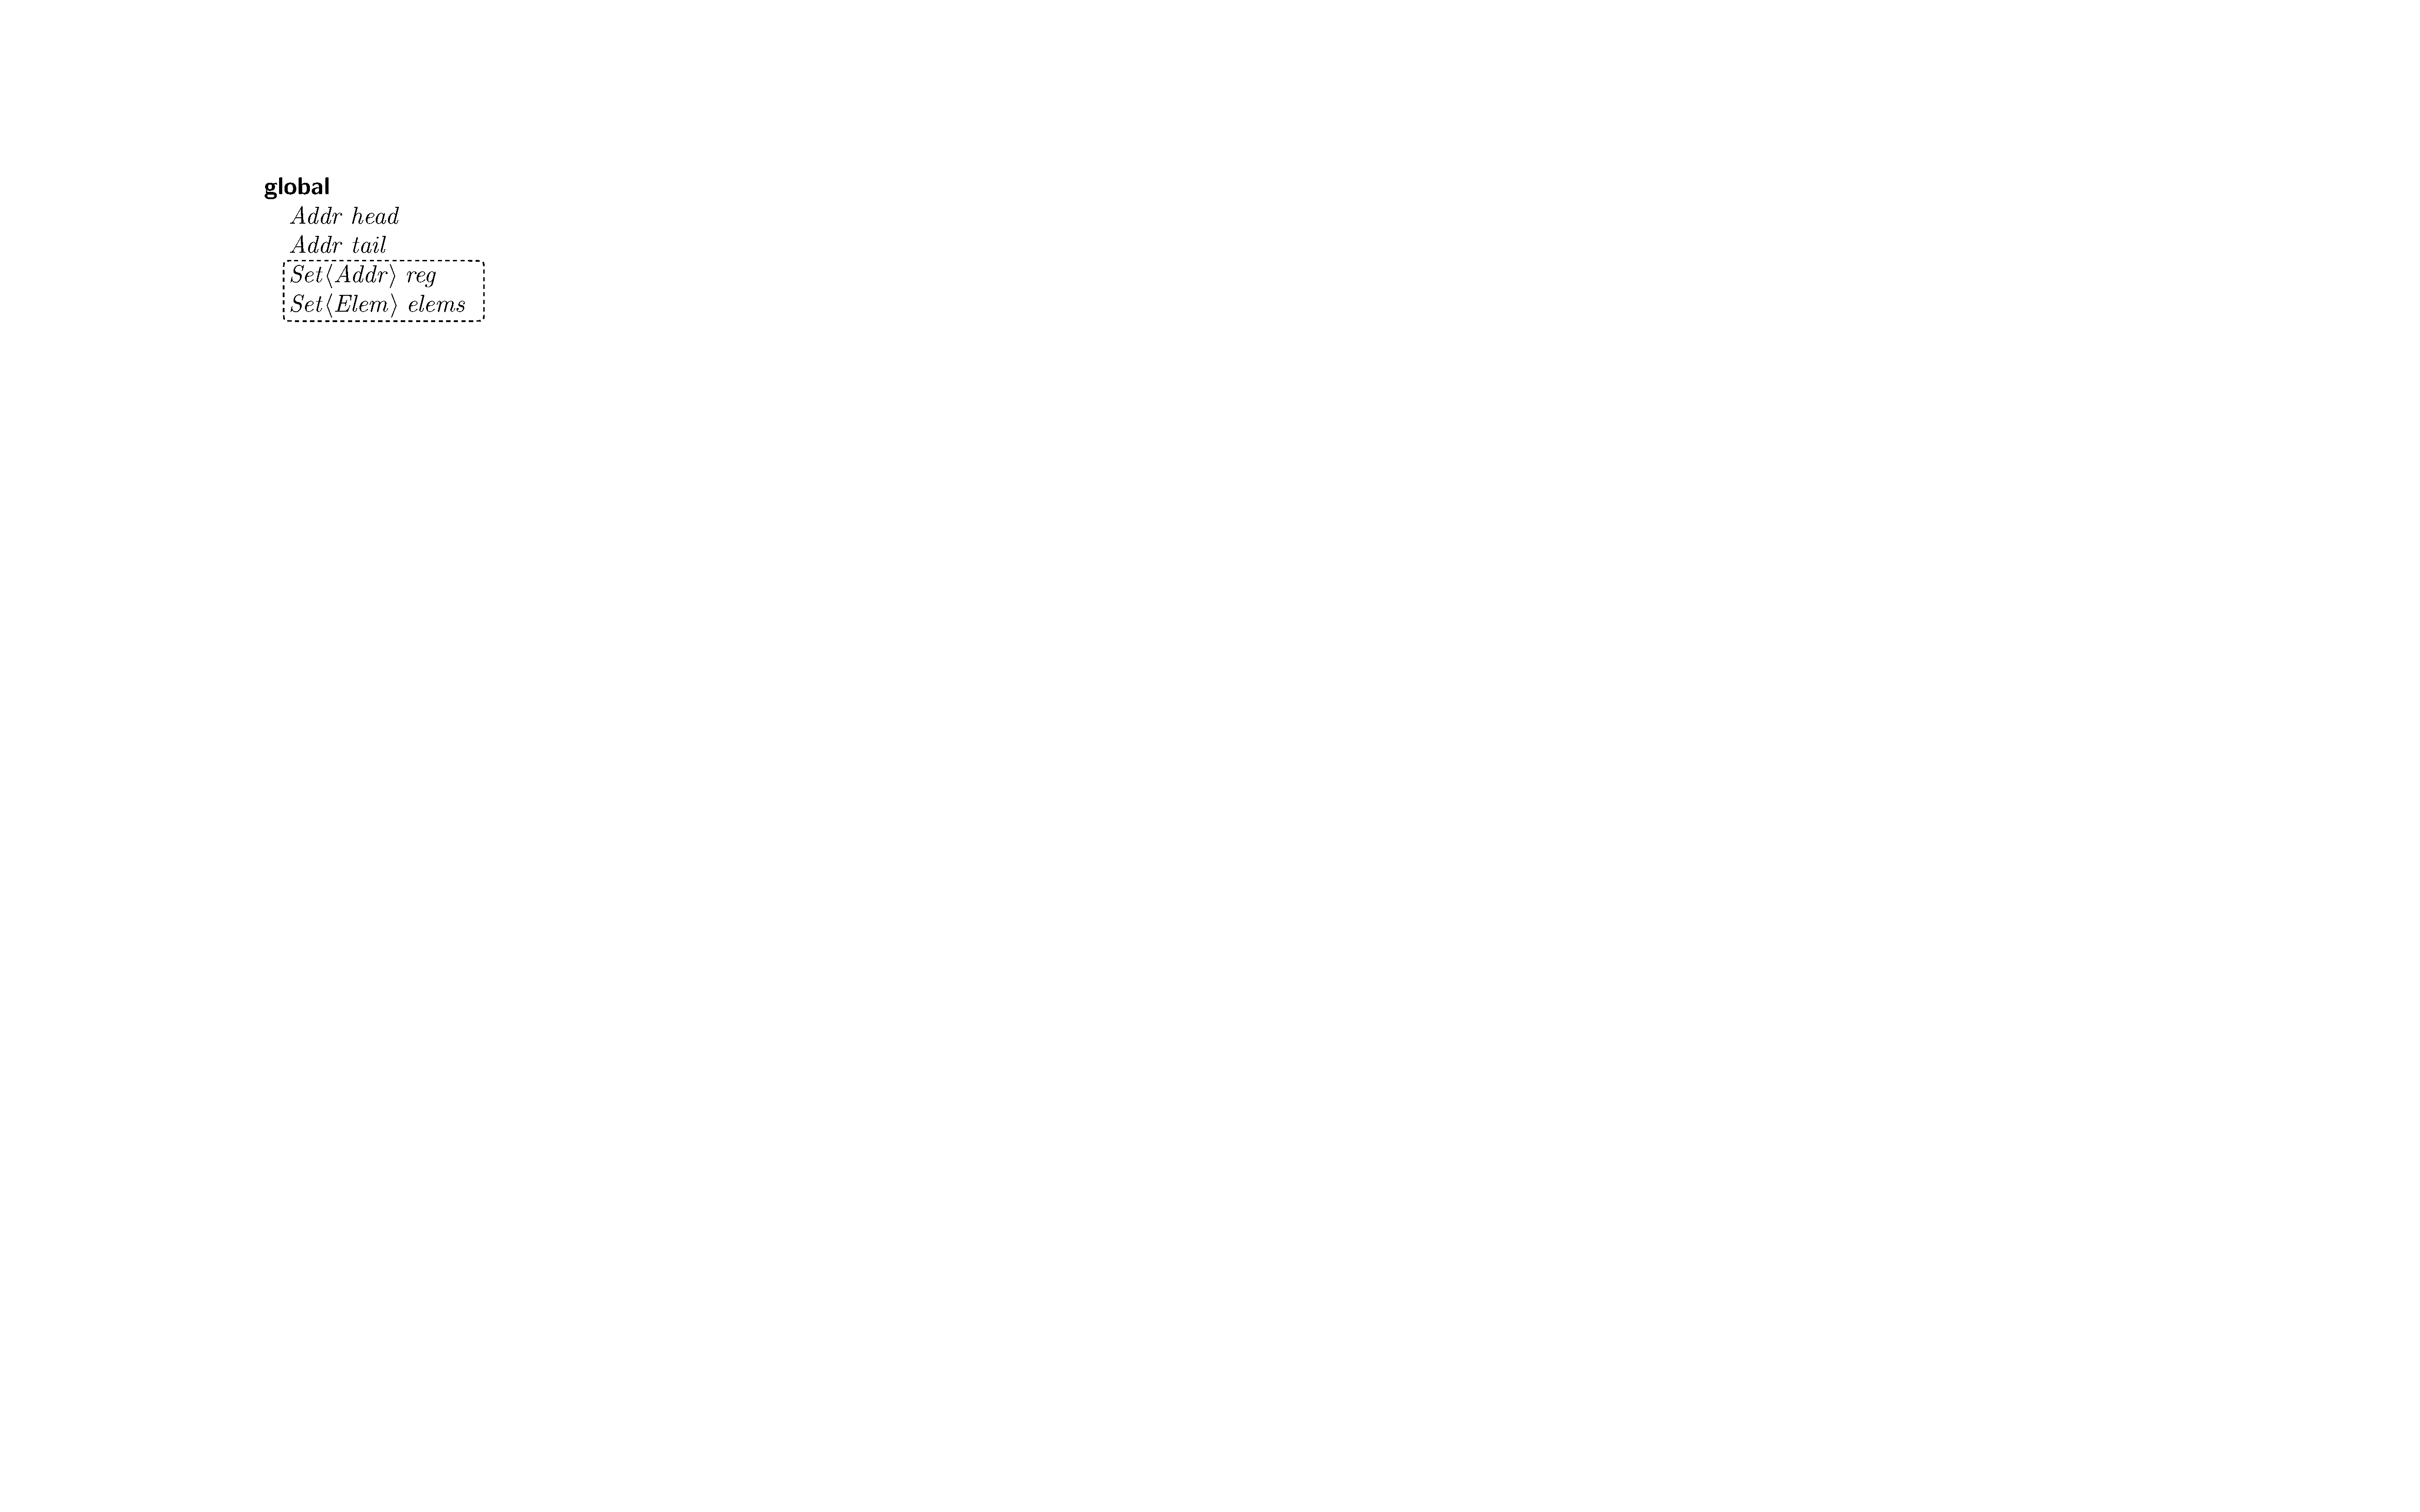
\includegraphics[scale=\figscale]{graphics/_lists_classes}
\end{center}
%
The declared global program variables are:

\head, an address, which points to the first node of the list which has the lowest possible value ($-\infty$).

\tail, an address, which points to the last node of the list  which has the lowest possible value ($+\infty$).

\region, a set of addresses, which is used to keep track of the portion of the heap whose cells form the list.

\elements, a set of elements, which represents the collection of elements stored in the list.

In figure \ref{fig:listcode} we present the program we are going to use, written in \gls{SPL}, with . We can see there are three procedures, \Search, \Insert and \Remove. 

We consider \head and \tail sentinel nodes which are neither removed nor 
modified and we assume that the list is initialized with \head and \tail 
already set.
%
The set \region is initialized containing solely the addresses of \head 
and \tail.
%
Similarly, the set \elements is initialized containing only the elements 
initially stored at the nodes pointed by \head and \tail.
%
There is also a function \concept{havocListElem}() which returns a random element. 


\begin{figure}[!htbp]
		\myframe{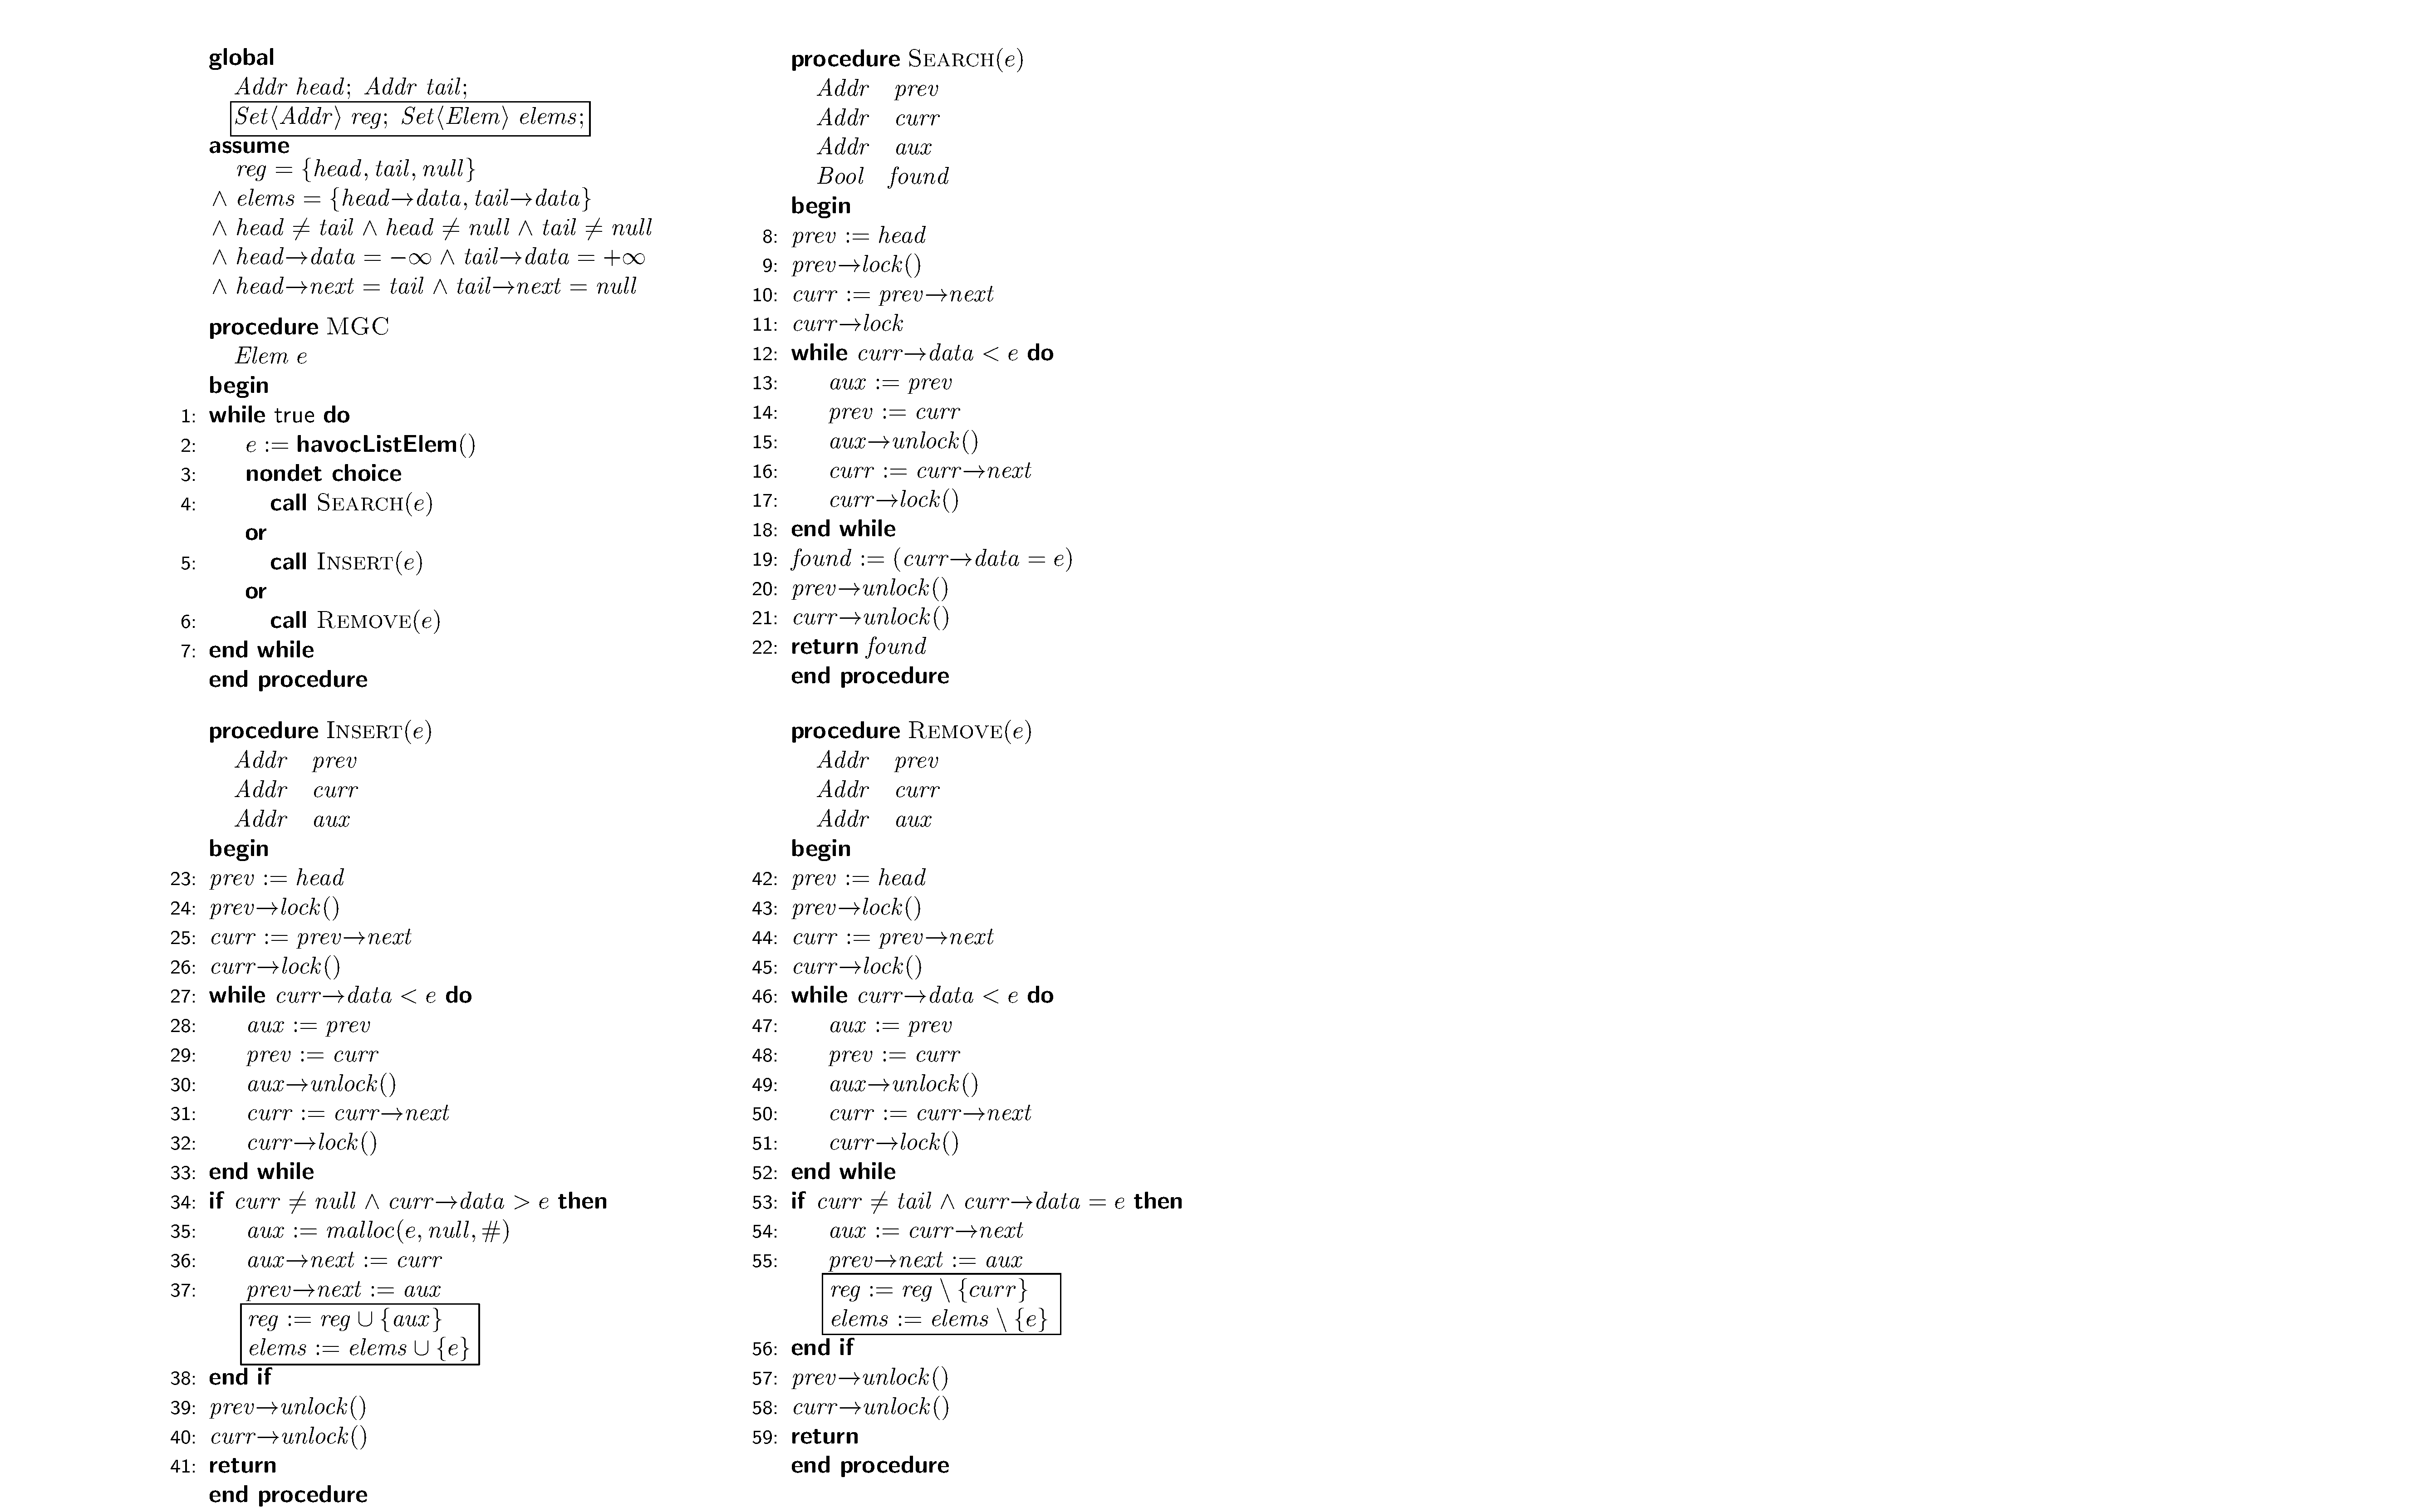
\includegraphics[scale=0.4]{graphics/_listcode}}
		\caption{Concurrent lock-coupling lists implementation.}
		\label{fig:listcode}
\end{figure}


\subsection{TL3}

\emph{Theory of Linked Lists with Locks} \TLLpL, is the theory we use for describing linked-list heap memory layout.
%
\TLLpL is a multi-sorted first-order theory.
%
It is multi-sorted because it has multiple types for its variables (address, element,...).
%
It is a first-order theory because only variables are quantifiable, as \gls{FOL}.

In this section \TLLpL is defined with the purpose we have. 
%
A more complete and formal definition of \TLLpL can be found in \citeapos{paperAle} and \citep[6.2]{thesisAle}.

Although some functions are originally defined \citep{thesisAle} in suffix notation (\fNext field for instance), preffix-notation has been used to described the theory. 
%
The reason for this modification is to be consistent with \spass syntax.
%
Furthermore, a subset of \TLLpL has been used. 
%
In the same way \gls{FOL} can be expressed with $\neg,\vee$ but sometimes $\implies$ is included but $\dimplies$ is not,
%
few functions have not been used because they can be expressed using others functions in the theory. 
%
We proceed to describe \TLLpL.


\TLLpL is a compound of theories. The \textbf{sorts} used among this theories are: 
%
\cell (representing the nodes of the list),
%
\elem (representing elements),
%
\addr (representing address),
%
\tid (representing thread id),
%
\mem (representing the memory also called heap. It is represented as maps of \addr to \cell ),
%
\path (representing a finite sequence of address),
%
\sSetWhatever (representing a set of \tid,\addr or \elem).

For each sort, there is a theory containing its constants, functions and predicates. 
%
There is one more theory, $\Sigma_{Bridge}$ is a \emph{bridge theory} containing auxiliary
functions, for example, that allow to map paths of addresses to set of 
addresses, or to obtain the set of addresses reachable from a given 
address following a chain of \fNext fields.



\subsection{Signature}

We proceed to describe the signature of each theory, listing the sorts used and explaining its functions, predicates and constants. 
%
Every theory includes the equality theory \ref{theory:equality} 


%%%%%%%%%%%%%%%%%%%%%%%%%%%%%%%%%%%%%%%%%%%%%%%%

%					TID 

%%%%%%%%%%%%%%%%%%%%%%%%%%%%%%%%%%%%%%%%%%%%%%%%
\begin{center}\rule{4cm}{0.4pt} $\Sigma_{\tid}$ \rule{4cm}{0.4pt}\end{center}
%
The sort used is \tid. The "no-thread" value is represented with \fNoThread.
%
Apart from the equality theory, this theory does not have any other predicates or functions.


%%%%%%%%%%%%%%%%%%%%%%%%%%%%%%%%%%%%%%%%%%%%%%%%

%					ELEM

%%%%%%%%%%%%%%%%%%%%%%%%%%%%%%%%%%%%%%%%%%%%%%%%


\begin{center}\rule{4cm}{0.4pt} $\Sigma_{\elem}$ \rule{4cm}{0.4pt}\end{center}
%
The sort used is \elem. 
%
There is a total order which allows to order every set of \elem.
%
In addition, this sort is upper and lower bounded.
%
The signature is described \doubt{in/at} table \ref{table:elem_signature}.


\begin{table}[hbtp]
\centering
\begin{tabular}{rrl}
\fHighest & \elem & Maximum value an \elem can take.\\
\fLowest & \elem & Minimum value an \elem can take.\\
\hline\hline
\fLselem & \elem$\times$\elem & Total order relation between \elem.
\end{tabular}
\caption{\textbf{Signature of $\Sigma_{\ensuremath{\mathit{elem}}}$.} Top block contains functions, lower block contains predicates.}
\label{table:elem_signature}
\end{table}


%%%%%%%%%%%%%%%%%%%%%%%%%%%%%%%%%%%%%%%%%%%%%%%%

%					CELL

%%%%%%%%%%%%%%%%%%%%%%%%%%%%%%%%%%%%%%%%%%%%%%%%

\begin{center}\rule{4cm}{0.4pt} $\Sigma_{\cell}$ \rule{4cm}{0.4pt}\end{center}
%
The sorts used are \cell,\elem,\addr,\tid.
%
The signature is described \doubt{in/at} table \ref{table:cell_signature}.

\begin{table}[hbtp]
\begin{tabular}{rrl}
\fMkcell & $\elem\times\addr\times\tid \to \cell$ & Constructor\\
\fNext & $\cell \to \addr$ & Getter of \fNext field \\ 
\fData & $\cell \to \elem$ & Getter of \fData field \\ 
\fLockID & $\cell \to \tid$ & Getter of \fLockID field \\ 
\fLock & $\cell\times\tid\to\cell$ & Construct a new \cell with \fData and \fNext \\
&&\;\;\;								values of the given \cell, \\
&&\;\;\;				using the \tid for the \fLockID field.\\
\fError & $\cell$ & Constant value used to model \\ 
&&\;\;\;				incorrect memory deference.
\end{tabular}
\caption{\textbf{Functions of $\Sigma_{\cell}$} theory.}
\label{table:cell_signature}
\end{table}

The function \fUnlock could be considered. Actually, \cite{thesisAle} includes it in the theory but it has not been included in this work.
%
The reason is justified because to \fUnlock a \cell is equivalent to \fLock a \cell with \fNoThread value.



%%%%%%%%%%%%%%%%%%%%%%%%%%%%%%%%%%%%%%%%%%%%%%%%

%					MEMORY

%%%%%%%%%%%%%%%%%%%%%%%%%%%%%%%%%%%%%%%%%%%%%%%%


\begin{center}\rule{4cm}{0.4pt} $\Sigma_{\mem}$ \rule{4cm}{0.4pt}\end{center}
%
The sorts used are \mem,\cell and \addr. 
%
The functions are described \doubt{in/at} table \ref{table:memory_signature}.

\begin{table}[hbtp]
\begin{tabular}{rrl}
\fNull & $\addr$ & Null address \\
\fRd & $\mem\times\addr\to\cell$ & Models memory deference. \\
&&								\;\;\; Returns the value from the \mem the \cell \\
&&								\;\;\; stored in the \addr.\\
\fUpd & $\mem\times\addr\times\cell\to\mem$ & Creates a new \mem from the given one
\end{tabular}
\caption{\textbf{Functions of $\Sigma_{\mem}$} theory}
\label{table:memory_signature}
\end{table}

%%%%%%%%%%%%%%%%%%%%%%%%%%%%%%%%%%%%%%%%%%%%%%%%

%					SETADDR

%%%%%%%%%%%%%%%%%%%%%%%%%%%%%%%%%%%%%%%%%%%%%%%%


\begin{center}\rule{4cm}{0.4pt} $\Sigma_{\sSetAddr}$ \rule{4cm}{0.4pt}\end{center}
%
It models the usual set theory. 
%
Preffix version of each function and predicate has been preferred to be consistent with \ref{ax::fulllist}.
%
The signature is described \doubt{in/at} table \ref{table:setaddr_signature}.

Intersection function and subset predicate has not been included despite \citep{thesisAle} uses them. 
%
They were not used because they were unnecessary.

\begin{table}[hbtp]
\begin{tabular}{rrl}
\fEmptyset & \sSetAddr & Empty set\\
\fSingl & $\addr\to\sSetAddr $& Constructor of a single-element set.\\
\fUnion & $\sSetAddr\times\sSetAddr\to\sSetAddr$&\\
\fSetdiff & $\sSetAddr\times\sSetAddr\to\sSetAddr$&\\
\hline\hline
\pIn & $\sAddr\times\sSetAddr $& \\
\end{tabular}
\caption{\textbf{Signature of $\Sigma_{\sSetAddr}$.} Top block contains functions, lower block contains predicates.}
\label{table:setaddr_signature}
\end{table}


%%%%%%%%%%%%%%%%%%%%%%%%%%%%%%%%%%%%%%%%%%%%%%%%

%					SETELEM

%%%%%%%%%%%%%%%%%%%%%%%%%%%%%%%%%%%%%%%%%%%%%%%%


\begin{center}\rule{4cm}{0.4pt} $\Sigma_{\sSetElem}$ \rule{4cm}{0.4pt}\end{center}
%

Again, it models the usual set theory.
%
The signature is described \doubt{in/at} table \ref{table:setelem_signature}.

\begin{table}[hbtp]
\begin{tabular}{rrl}
\fEmptysetElem & $\sSet $& Empty set\\
\fSinglElem & $\elem\to\sSet $& Constructor of a single-element set.\\
\fUnionElem & $\sSet\times\sSet\to\sSet$&\\
\fSetdiffElem & $\sSet\times\sSet\to\sSet$&\\
\hline\hline
\pInElem & $\sAddr\times\sSet $& \\
\end{tabular}
\caption{\textbf{Signature of $\Sigma_{\sSet}$.} Top block contains functions, lower block contains predicates.}
\label{table:setelem_signature}
\end{table}


%%%%%%%%%%%%%%%%%%%%%%%%%%%%%%%%%%%%%%%%%%%%%%%%

%					SETTID

%%%%%%%%%%%%%%%%%%%%%%%%%%%%%%%%%%%%%%%%%%%%%%%%


\begin{center}\rule{4cm}{0.4pt} $\Sigma_{\sSetTid}$ \rule{4cm}{0.4pt}\end{center}
%


The signature is described \doubt{in/at} table \ref{table:settid_signature}.

\begin{table}[hbtp]
\begin{tabular}{rrl}
\fEmptysetTid & $\sSetAddr $& Empty set\\
\fSinglTid & $\addr\to\sSetAddr $& Constructor of a single-element set.\\
\fUnionTid & $\sSetAddr\times\sSetAddr\to\sSetAddr$&\\
\fSetdiffTid & $\sSetAddr\times\sSetAddr\to\sSetAddr$&\\
\hline\hline
\pInTid & $\sAddr\times\sSetAddr$ &\\
\end{tabular}
\caption{\textbf{Signature of $\Sigma_{\sSetAddr}$.} Top block contains functions, lower block contains predicates.}
\label{table:settid_signature}
\end{table}

